\documentclass[a4paper]{article}
\setlength{\oddsidemargin}{0in}
\setlength{\evensidemargin}{0in}
\setlength{\textwidth}{160mm}
\setlength{\topmargin}{-15mm}
\setlength{\textheight}{240mm}
\usepackage{graphicx}

\begin{document}
	\title{CS26020 Assignment \\ Developing a Maze Exploring Robot Controller \\ Project Report}
	\author{Rhys Evans (rhe24@aber.ac.uk)}
	\date{25th April 2018}
	\maketitle
	\newpage
	\tableofcontents
	\newpage
	
	\section{Introduction}
	The objective of this project was to create a robot controller capable of exploring a perfect maze. This was accomplished by combining reactive and deliberative robotic behaviours, thus creating a 'hybrid' system. In this report I will discuss and evaluate the process of designing, implementing and testing the controller, along with the challenges I faced. In addition, I will discuss any changes I would make to the system if done again.
	
	\section{Design Analysis}
	In this section I will analyse various aspects of the controller's design and discuss some of the decisions I made when designing the system.
	
	\subsection{Modelling The Maze}
	Arguably the most important aspect of this controller is the maze model, without a reliable maze model there is no basis for the deliberative behaviour of the controller. I decided to use a fairly simple 2D Array of cells to represent the maze. I felt this was a sufficiently simple method, as the robot's starting point would always be at (1, 0) in this representation. It would also make indexing the maze (a common occurance) very easy.
	
	\subsection{Modelling The Robot}
	Having already decided on a method to store the maze I also needed to put some thought into representing the robot within the maze in a way that supported the maze model. I came to the conclusion that in order to fully encapsulate the robot I needed to store the following information:\\
	
	\begin{itemize}
		\item The robot's position within the maze (X and Y)
		\item The robot's orientation (North, West, South East), relative to the maze.
		\item The number of cells the robot has visited\\
	\end{itemize}
	
	
	\subsection{Navigating The Maze}
	Now that I had a model in mind for both the robot and the maze it was easier to think about how the robot would use its hybrid behaviour to navigate the maze. Firstly I decided on how the robot would fully explore the maze, I settled on the 'left hand rule'. This would mean that at each given cell the robot's preference of direction would be as follows:\\
	
	\begin{enumerate}
		\item Turn Left
		\item Go Forward
		\item Turn Right
		\item Turn Around\\
	\end{enumerate}
	
	If the first option is unavailable, attempt the second and so on.\\ 
	
	In order for the robot to implement the 'left hand rule', the maze model must be populated with the information required. This was done by enforcing a specific order of operations for the robot. For each cell the robot visits the following operations should be carried out:
	
	\newpage
	
	\begin{enumerate}
		\item \textbf{Detect}
		\begin{itemize}
			\item Use the robot's IR sensors to detect and store the walls of the cell
			\item Take light level readings and decide if the current cell is the nest cell
			\item Increase the number of cells visited and check if the robot has explored all 16 cells, if so indicate completion
		\end{itemize}
		\item \textbf{Turn}
		\begin{itemize}
			\item Use the information gathered in the above step to decide on the new direction (using left hand rule)
			\item If needed, turn the robot to face the correct direction
			\item Update direction of robot
		\end{itemize}
		\item \textbf{Drive}
		\begin{itemize}
			\item Drive forward and avoid obstacles using reactive behaviours
			\item If black line is encountered on the cell floor, return to step 1.
		\end{itemize}
	\end{enumerate}
	
	\subsection{Drawing The Maze}
	This is an extra feature specified in the project brief that I decided to implement, the maze is drawn on the robot's LCD screen using line plots. As my maze is modelled as a 2D Array I felt it would be reasonable to represent the maze in a 28x28 pixel region of the screen, with each cell of the maze being 7x7 pixels. The LCD screen is 127x31 pixels, therefore 28 is the largest multiple of 4 (height of the maze) that could appropriately represent the maze.\\
	
	\section{Implementation}
	In this section I will discuss and evaluate my implementations of system's design and any challenges that had to be overcome. 
	
	\subsection{The Maze Model}
	I decided to implement the 2D array of cells by declaring a 'Cell' structure with two attributes: 'visited' and 'walls'. The 'visited' attribute is simply a boolean to store whether or not the cell has already been explored. The 'walls' attribute is a boolean array of 4 elements to represent the four walls of the maze (0 if no wall is present, 1 if wall is present). Lastly there is a single global variable of type 'Cell' to store the 'nest cell'.
	
	\subsection{The Robot Model}
	In order to implement my representation of the robot I simply created 4 variables:
	\begin{itemize}
		\item int currentDirection
		\item int currentPosX
		\item int currentPosY
		\item noVisitedCells
	\end{itemize}
	
	I considered using a structure to represent the robot and store these variables, however as it would only have a single instance I decided to opt for the simplest solution. To aid in the readability of the code I used preprocessor variables for directions.
	
	\subsection{Navigating The Maze}
	This was the most time consuming aspect of the controller's development, in order to combine the reactive and deliberative behaviours necessary to navigate the maze I used a single finite state machine. The state machine is comprised of 5 states:
	
	\begin{itemize}
		\item Start   - Initialization of the system 
		\item Detect  - Updating the overall model
		\item Turn    - Turning the robot based on the model
		\item Drive   - Moving the robot from cell to cell and avoiding obstacles
		\item Finish  - Indicating completion and allowing for restart
	\end{itemize}
	
	I chose these states based on the different behaviours of the robot and the necessary operations to explore the maze. Each state has a corresponding function within the program that is only called once from within a switch-case statement in the main loop. Each function performs the operations associated with that state repeatedly until the state is changed.\\
	
	The system stores the current state in a global variable, which is only changed through a 'changeState()' function. Use of this function allows 'one-time-only behaviours', for example when the Finish state is entered a short tune plays just once through this function. State changes are triggered by certain events within the current state, this is illustrated in the below State Machine Diagram:
	
	\begin{figure}[!htb]
		\centering
			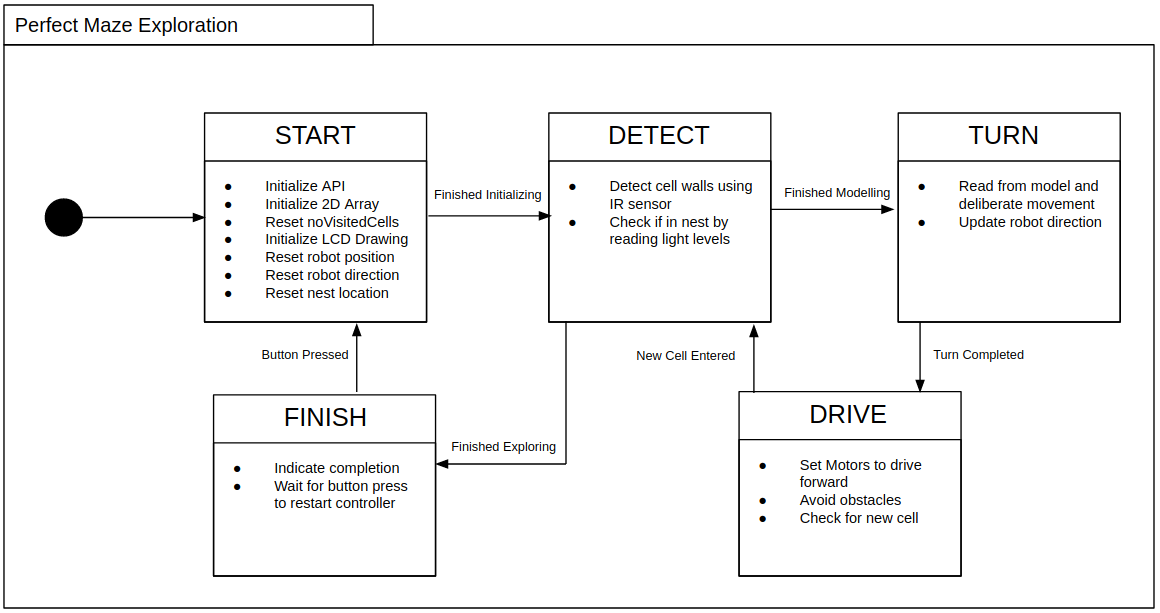
\includegraphics[width=0.75\linewidth]{./img/smd.png}
			\caption{State Machine Diagram}
			\label{fig:state-diagram}
	\end{figure}
	
	The reactive aspect of the robot's behaviour is implemented in the obstacle avoidance function within the 'Drive' state. It allows the robot to correct its position and prevent itself from colliding with the walls by using the IR sensors on the left and right side of the robot.\\
	
	The robot must be able to detect cell changes in order to advance the state machine, this is done by checking for a very small reading from underside IR sensors of the robot. When a sufficiently small reading is detected the controller delays for 500ms then stops the robot and advances the state. The purpose of the 500ms delay is to allow the robot to continue creeping all the way into the cell before stopping and to ensure no false-positive readings from the line sensors. Although it would probably have been better practice to use a timing system. I felt that the delay was short enough that it wouldn't obstruct any of the robot's behaviours.
	
	\newpage
	
	\subsection{Drawing The Maze}
	At first glance, implementing the maze drawing based on the design specified seemed straightforward. However, one issue I overlooked was the difference in coordinates between the 2D Array and the LCD Screen. (0, 0) on the LCD Screen is on the top left, whereas it is in the bottom left in the Maze Model. To solve this problem I inverted the Y axis of the LCD screen when drawing.\\
	
	To draw the maze, the 2D Array is iterated over twice with nested for-loops, the first pair of for-loops simply draws the border walls of the maze. The second, larger for-loop draws all the walls within the maze and plots the robot's position within the maze. The maze drawing all happens within a drawMaze() function, which is called every time the robot enters a new cell, in order to update the drawing. Below is an image of a completed maze being drawn on the LCD: 
	
	\begin{figure}[!htb]
		\centering
			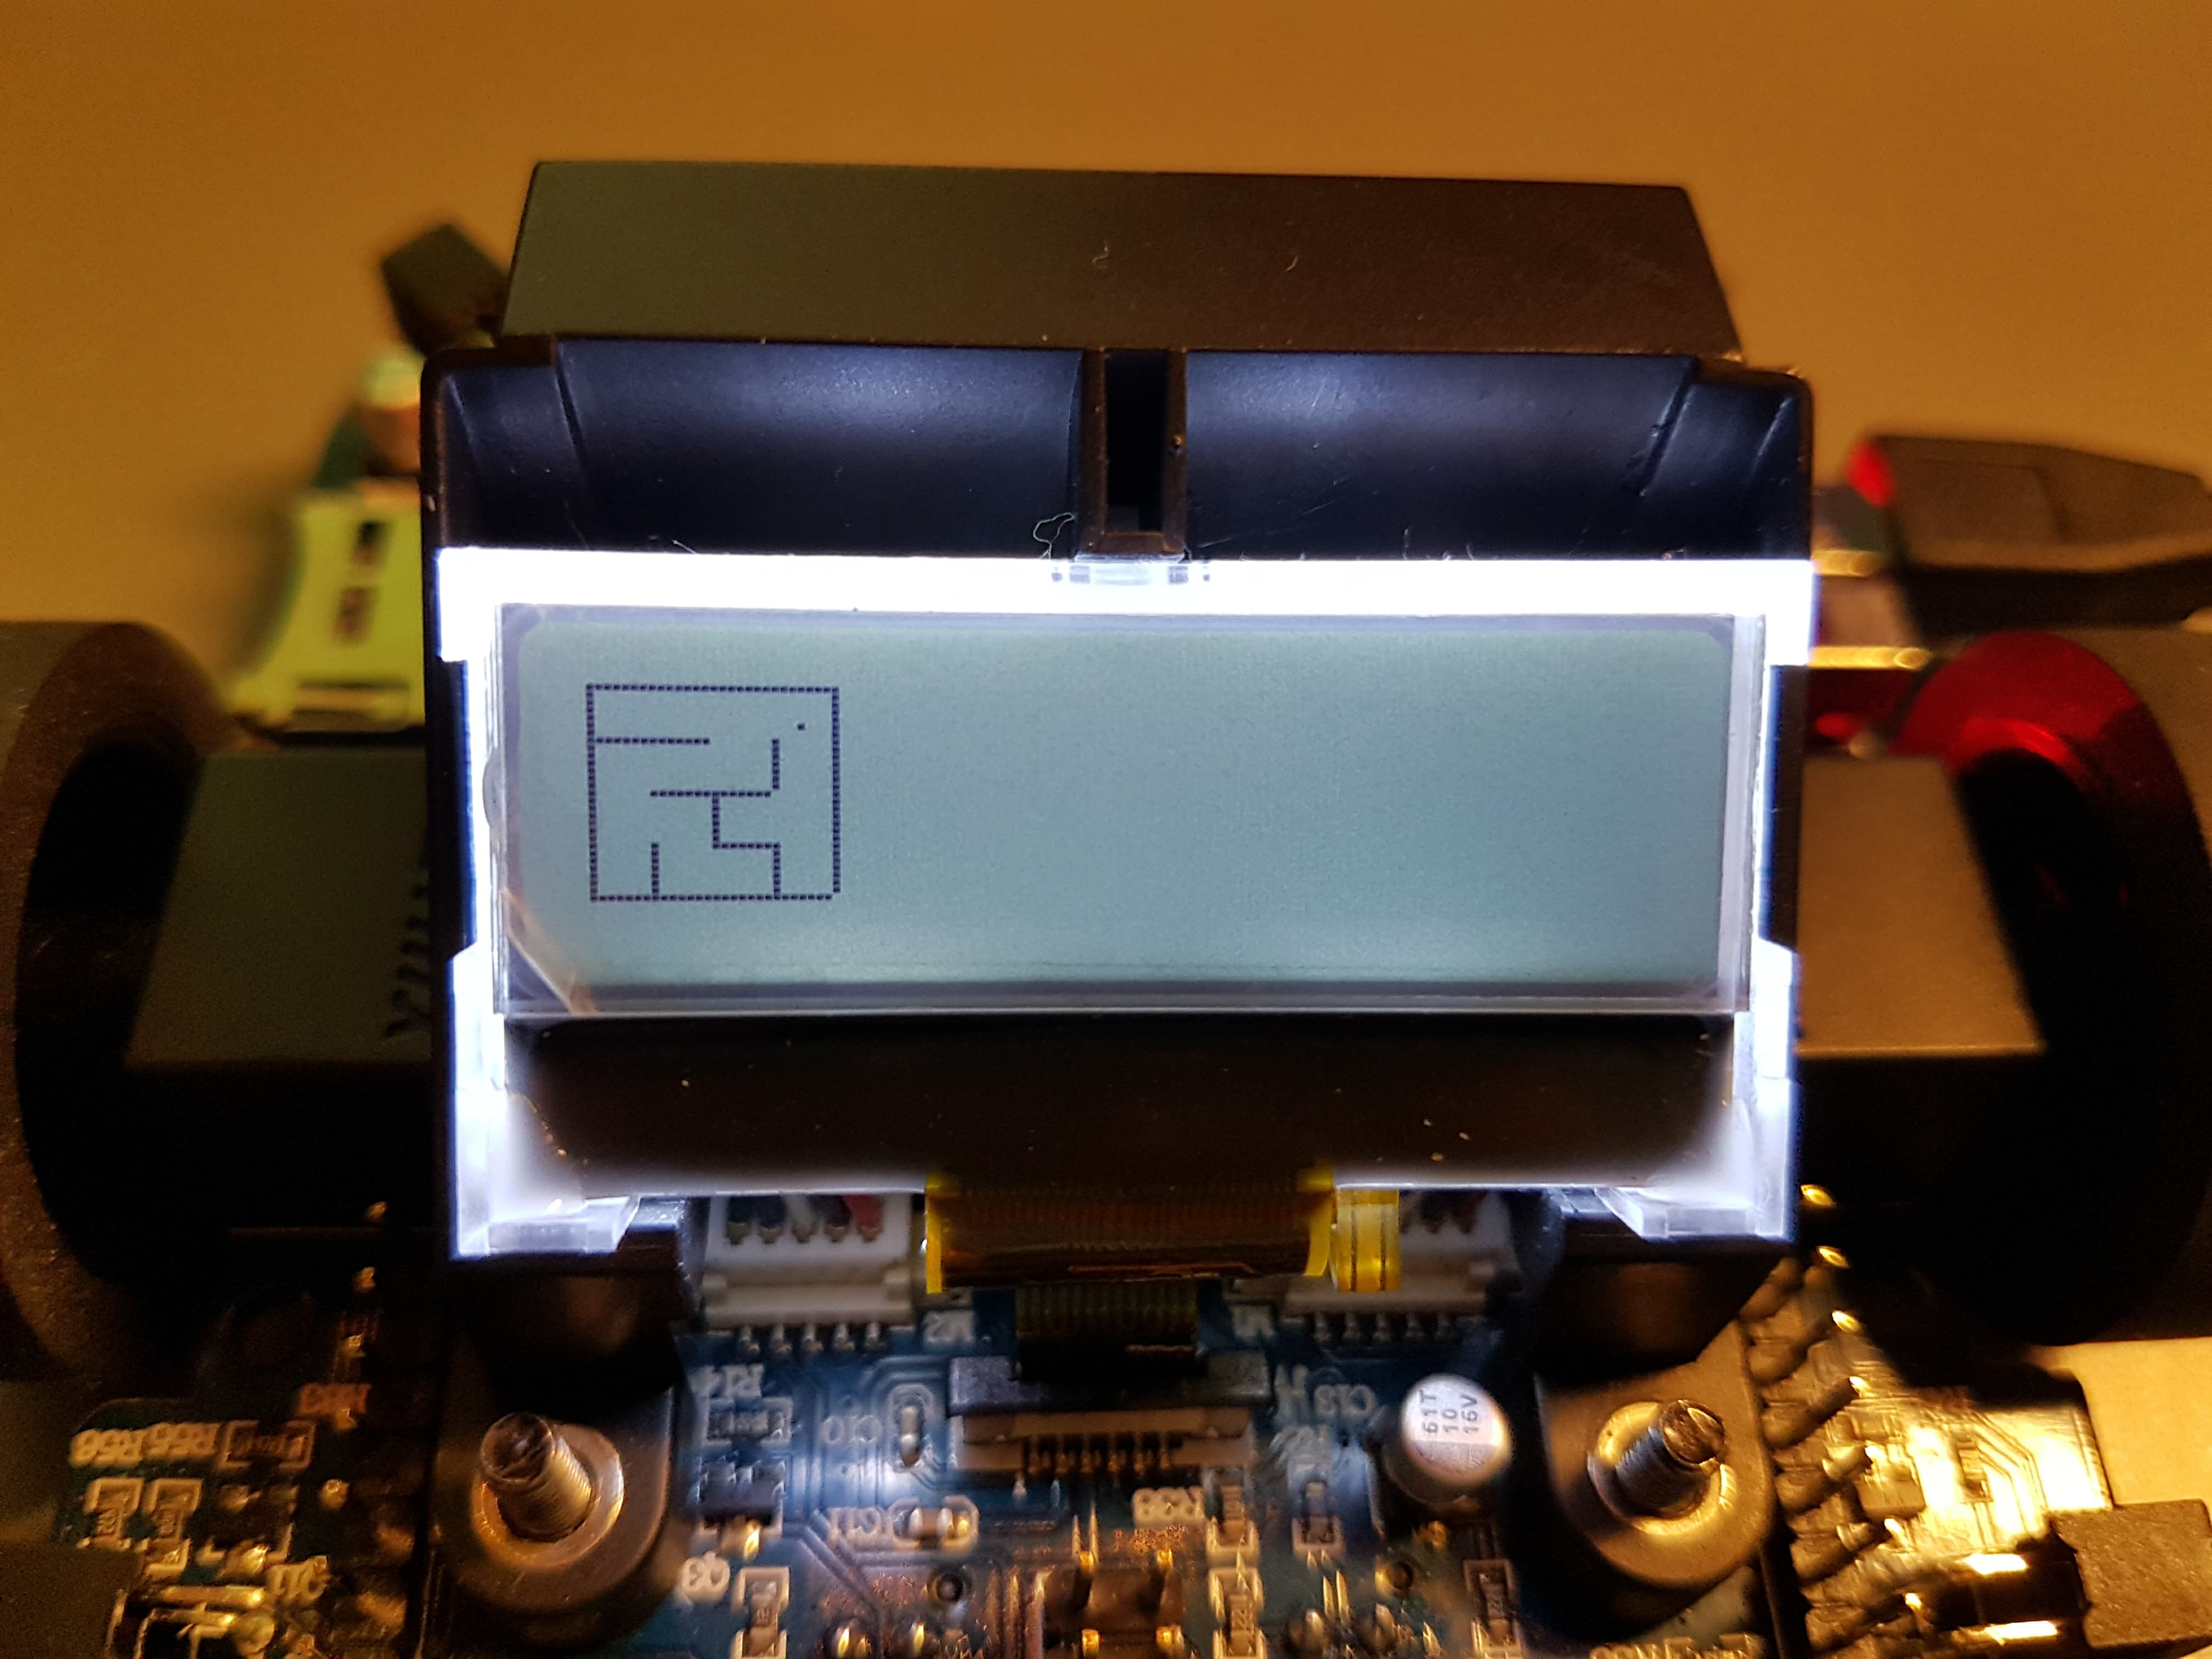
\includegraphics[width=0.5\linewidth]{./img/maze.jpg}
			\caption{Maze Represented on LCD Screen}
			\label{fig:maze-draw}
	\end{figure}
	
	\section{Testing}
	One of the biggest differences I noticed between programming for an embedded system versus a non-embedded system was the testing and debugging process. Although the bluetooth connection proved very helpful to debug certain issues during testing I still found myself spending more time than usual solving simple problems. If I were to undertake a project like this again in the future, I would test more frequently and try to implement less features between each test.\\
	
	To support debugging in my controller I have implemented a printDebugStream() function to send debug information through bluetooth. This function is called within a preprocessor ifdef statement each time the robot enters a new cell. Using the preprocessor for this allowed me to quickly enable or disable debugging within the system, this proved very helpful when testing the functionality of the controller.
	
	\newpage
	
	\section{Evaluation and Improvements}
	I feel that overall my hybrid controller makes a good attempt at solving the maze exploration problem. My maze model was able to support the deliberative behaviour of the robot and effectively map the maze and the obstacle avoidance within my controller enabled to robot to behave reactively. I was also able to implement the representation of the maze on the LCD Screen.\\
	
	The parts where I feel my controller didn't perform as well as expected was recovering and correcting properly after a turn. Often times the robot would take turnings too sharply or not sharply enough, this would lead to bad positioning, in some cases it would hinder the IR sensors' ability to detect and lead to an inaccurate model. Turnings that were left un-corrected would cause the problem to grow at each cell advancement as the robot would veer further off course and continue to behave unpredictably. If I were to undertake this project again I would put more effort into ensuring the robot corrects its position after each turning.\\
	
	Due to the problems listed above I decided against implementing the return-to-nest feature, as I felt the successful exploration was more important and needed my focus. However if I were to have implemented this feature I would have deliberated between the two methods described below.
	
	\subsection{Inverted Turning Logic}
	This is probably the simplest solution for returning to the nest area, it simply involves inverting the logic used to decide on the robot's turning direction. In my system I chose to use the 'left hand rule' to explore the maze, therefore to return to the nest I would simply opt for the 'right hand rule' instead until the nest area was encountered again. Although this solution is very simple it is not very efficient, in order to find the nest again the robot could potentially visit every cell before it finds the nest again.\\
	
	To implement this method I would likely introduce another finite state machine into the system that would split the 'drive' or 'turn' state into two other sub-states, 'explore' and 'return'. These two states would dictate the robot's decision making.
	
	\subsection{The 'Breadcrumbs' Method}
	This method is considerably less simple than the above, however it should always find the shortest route back to the nest, thus making it more efficient. To implement this method I would have introduced a new state machine as above, that splits the drive state into three sub-states: 'pre-nest', 'post-nest' and 'return'. Each one causing a different behaviour, the 'pre-nest' would explore the maze as normal until the nest is found, then 'post-nest' would be entered. Whilst the system is in this state, the controller would incrementally leave a 'breadcrumb' at each new cell, this would be represented as an additional attribute in the 'Cell' structure. Once the maze is fully explored the system would enter the 'return' state, where it would scan all it's adjacent cells for the smallest numbered 'breadcrumb', then travel to that cell. The robot would continue with this method until the nest is encountered.
	
\end{document}